\documentclass[tikz,border=5pt]{standalone}
\usepackage{luatexja}
\usepackage[hiragino-pron]{luatexja-preset}
\usepackage{amsmath,amssymb,bm}
\usetikzlibrary{arrows.meta}

\begin{document}
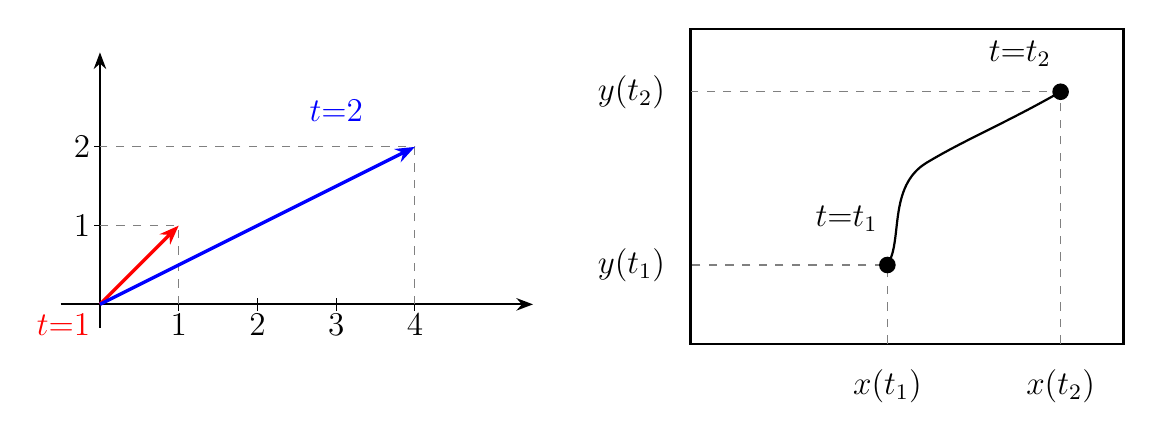
\begin{tikzpicture}[every node/.style={font=\large}]

  %% Left figure: position vectors at t=1 and t=2
  \begin{scope}
    \draw[-{Stealth[length=6pt]}, thick] (-0.5,0) -- (5.5,0);
    \draw[-{Stealth[length=6pt]}, thick] (0,-0.3) -- (0,3.2);

    % Tick marks
    \foreach \x in {1,2,3,4} {
      \draw (\x,0.08) -- (\x,-0.08);
      \node[below] at (\x,0) {$\x$};
    }
    \foreach \y in {1,2} {
      \draw (0.08,\y) -- (-0.08,\y);
      \node[left] at (0,\y) {$\y$};
    }

    % Dashed guides for t=1: (1, 1)
    \draw[dashed, gray] (1,0) -- (1,1) -- (0,1);

    % Dashed guides for t=2: (4, 2)... wait, let me think
    % u(t) = (t, t^2) doesn't work for these coordinates
    % From the image: at t=1 roughly (1, 0.7), at t=2 roughly (4, 2)
    % This looks like u(t) = (t^2, t) or similar? Actually no.
    % Image shows: t=1 arrow to about (1, 0.7), t=2 arrow to (4, 2)
    % Let me just match the image visually

    \draw[dashed, gray] (4,0) -- (4,2) -- (0,2);

    % Position vector at t=1
    \draw[-{Stealth[length=7pt]}, very thick, red] (0,0) -- (1,1);
    \node[red, below left] at (0,0) {$t{=}1$};

    % Position vector at t=2
    \draw[-{Stealth[length=7pt]}, very thick, blue] (0,0) -- (4,2);
    \node[blue, above] at (3,2.2) {$t{=}2$};

    \node[below left] at (0,0) {};
  \end{scope}

  %% Right figure: trajectory in xy-plane
  \begin{scope}[xshift=8cm]
    % Box (screen/plane)
    \draw[thick] (-0.5,-0.5) rectangle (5,3.5);

    % Axes labels
    \node[below] at (2,-0.7) {$x(t_1)$};
    \node[below] at (4.2,-0.7) {$x(t_2)$};
    \node[left] at (-0.7,0.5) {$y(t_1)$};
    \node[left] at (-0.7,2.7) {$y(t_2)$};

    % Dashed guides
    \draw[dashed, gray] (2,-0.5) -- (2,0.5) -- (-0.5,0.5);
    \draw[dashed, gray] (4.2,-0.5) -- (4.2,2.7) -- (-0.5,2.7);

    % Trajectory curve
    \draw[thick] (2,0.5) .. controls (2.2,0.8) and (2,1.5) .. (2.5,1.8)
      .. controls (3,2.1) and (3.5,2.3) .. (4.2,2.7);

    % Points
    \fill (2,0.5) circle (3pt);
    \node[above left] at (2,0.8) {$t{=}t_1$};

    \fill (4.2,2.7) circle (3pt);
    \node[above left] at (4.2,2.9) {$t{=}t_2$};
  \end{scope}

\end{tikzpicture}
\end{document}
